\documentclass{l4proj}


\usepackage{url}
\usepackage{amssymb}
\usepackage{graphicx}
\usepackage{algorithmic}
\usepackage[ruled,vlined]{algorithm2e}
\usepackage{amsthm}

\newtheorem{thm}{Theorem}
\newtheorem{definition}{Definition}
\newtheorem{lemma}{Lemma}


\begin{document}
\title{Diamond-free Degree Sequences}
\author{Alice Miller and Patrick Prosser}
\date{October 18, 2012}
\maketitle

\begin{abstract}
While attempting to classify partial linear spaces produced during the execution of an
extension of Stinson's hillwalking algorithm a new problem arises, that of generating all graphical degree sequences 
that are diamond-free (i.e. have no diamond as subgraph) and satisfy additional constraints.  
We present this problem (CSPLib 50), propose a constraint programming solution and list all
satisfying degree sequences of length 8 to 16 inclusive.
\end{abstract}

\educationalconsent
%
%NOTE: if you include the educationalconsent (above) and your project is graded an A then
%      it may be entered in the CS Hall of Fame
%
\tableofcontents
%==============================================================================

\chapter{Introduction}
\pagenumbering{arabic}
\label{sec:intro}
\vspace{-3mm}
We introduce a new problem, CSPLib number 50 \cite{CSPLib}, to generate all degree sequences that have a
corresponding diamond-free graph with secondary properties. This
arises naturally from a problem in mathematics to do with partial linear spaces; 
we devote a section of this paper to this. The problem itself is challenging with respect to 
computational effort arising from the large number of symmetries within the models. We introduce
two constraint programming models. The second model is an improvement on the first, and this improvement
largely consists of breaking the problem into three stages: the first stage produces degree sequences 
that satisfy arithmetic constraints, the second stage tests that a given degree sequence is graphical and if it is the third stage determines if
there exists a graph with that degree sequence that is diamond-free. We now present the problem in detail and
give motivation for it. Two models are then presented, along with a list of solutions. We then conclude and
suggest future work.

\chapter{Problem Definition}
\label{sec:probDefn}
\vspace{-3mm}
Given a simple undirected graph $G = (V,E)$, $V$ is the set of vertices and $E$ the set of undirected 
edges. The edge $\{u,v\} \in E$ if and only if vertex $u$ is adjacent to vertex $v$ in $G$. 
The graph is simple in that there are no loop edges, 
i.e. $\forall_{v \in V}~[\{v,v\} \notin E]$. Each vertex $v$ in $V$ has a degree 
$\delta(v) = |\{\{v,w\} : \{v,w\} \in E\}|$, i.e. the number of edges incident on that vertex.

A diamond is a set of four vertices in $V$ such that there
are  five edges between those vertices (see Figure \ref{fig:g1} for an example of a diamond). Conversely, 
a graph is diamond-free if it has no diamond as a subgraph, i.e. for every set of four vertices 
the number of edges between those vertices is at most four. Determining whether a graph is diamond-free is a polynomial-time
problem. E.g. checking every four vertices for a diamond is at worst case $O(n^{4})$.  
Note that a diamond is sometimes referred to as a $K_{4}-e$ graph.  
Our definition of a diamond-free graph agrees with that of \cite{lai} which addresses a different, but related problem. 
That is, identifying degree sequences for which there is a realisation containing a diamond as a subgraph. 
Others use the term diamond-free to denote a graph which has no diamond as an {\it induced} subgraph 
(in which case a $K_{4}$ is an allowable subgraph, unlike in our case).
A further definition of a diamond-free graph \cite{bast} is a graph $G$ with no diamond as a {\it minor}, i.e. a graph 
(isomorphic to one that can be) obtained from a subgraph of $G$ by zero or more edge contractions.

\begin{figure}
\centering
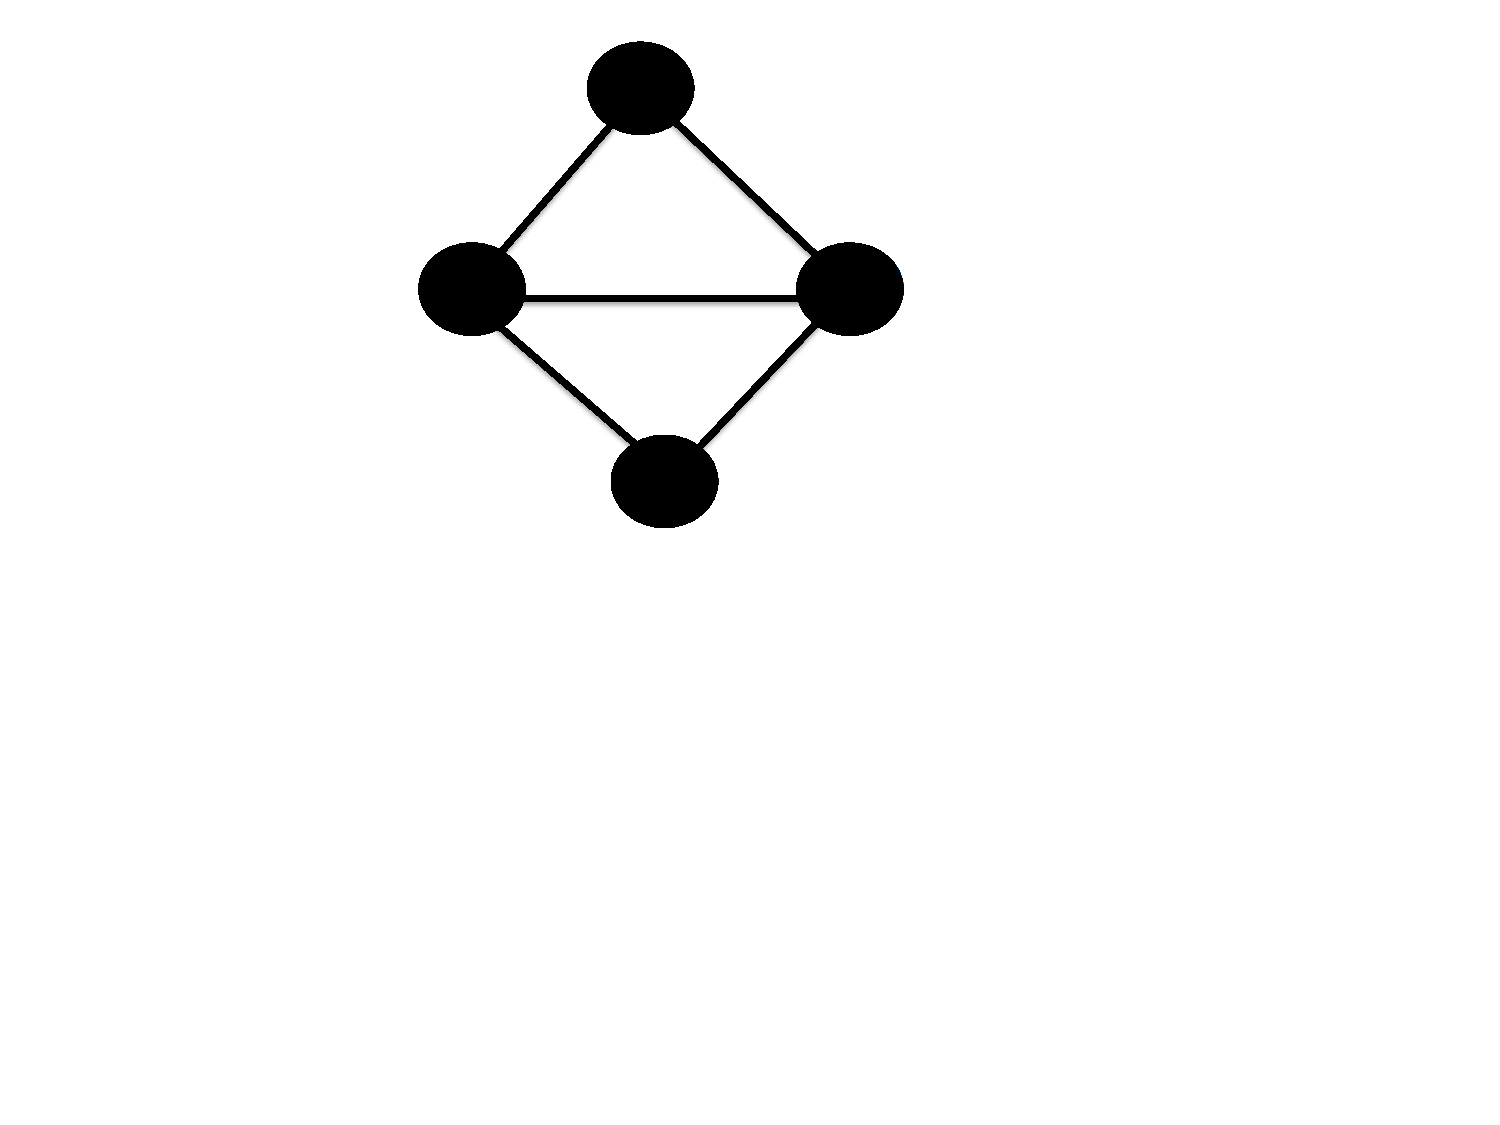
\includegraphics[height=8.0cm,width=9.0cm]{g1}
\vspace{-2cm}
\caption{A simple diamond graph of four vertices and five edges.}
\label{fig:g1}
\end{figure}

\begin{figure}
\centering
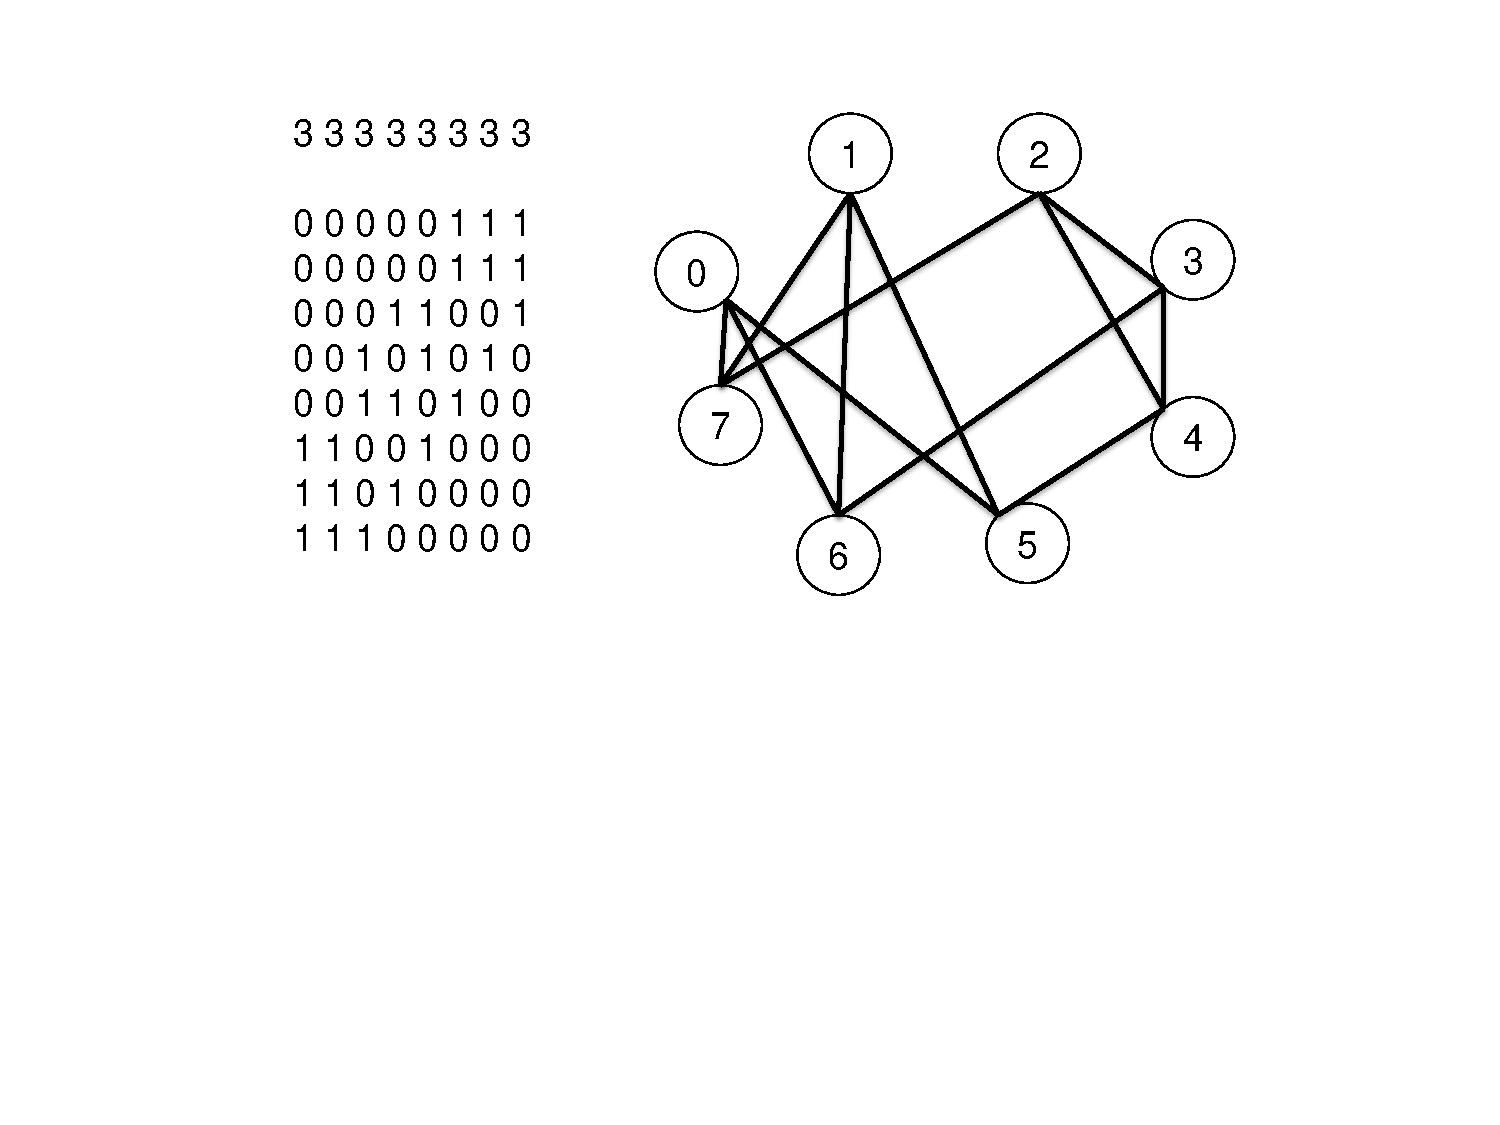
\includegraphics[height=8.0cm,width=12.0cm]{g8}
\vspace{-2cm}
\caption{Unique degree sequence for $n = 8$ with adjacency matrix and diamond-free graph.}
\label{fig:n8}
\end{figure}

In our problem we have additional properties required of the degree sequences of the graphs, in particular
that the degree of each vertex is greater than zero (i.e. isolated vertices are disallowed), the degree
of each vertex is divisible by 3 and the sum of the degrees is divisible by  12 (i.e. $|E|$ is divisible by  6).

The problem is then for a given value of $n$, such that $|V| = n$, produce all degree sequences 
$\delta(1) \geq \delta(2) \geq ... \geq \delta(n)$ such that there exists a diamond-free graph with that degree sequence,
each degree is non-zero and divisible by  3, and the number of edges is divisible by  6.
In Figure \ref{fig:n8} we give as an example the unique degree sequence for $n=8$ that satisfies our arithmetic constraints and 
is graphical, an adjacency matrix with that degree sequence and a corresponding simple graph that is diamond-free graph.

\chapter{Motivation}
\label{sec:motivation}
\vspace{-3mm}
The problem is a byproduct of attempting to classify
partial linear spaces that can be produced during the execution of an
extension of Stinson's hillwalking algorithm for block designs with
block size $4$ (see \cite{codihandbook}). First we need some definitions.
%\iffalse
\begin{definition}
A Balanced Incomplete Block Design (BIBD) is a pair $(V,B)$ where $V$
is a set of $n$ points and $B$ a collection of subsets of $V$ (blocks)
such that each element of $V$ is contained in exactly $r$ blocks and
every $2$-subset 
of $V$ is contained in exactly $\lambda$ blocks.
\end{definition}
%\fi

\noindent
Variations on $BIBD$s include {\it Pairwise Balanced Designs} (PBDs) in
which blocks can have different sizes, and {\it linear spaces} which
are PBDs in which every block has size at least $2$. It is usual to
refer to the blocks of a linear space as a {\it line}. A partial
linear space is a set of lines in which every pair appears in {\it at most}
$\lambda$ blocks. Here we refer to a BIBD with $\lambda=1$ as a {\it block design} and
to a partial linear space with $\lambda=1$, having $s_{i}$ lines of size $i$, where $i\geq 3$
and $s_{i}>0$ as a $3^{s_{3}}4^{s_{4}}\ldots$ structure.
For example, a block design on $7$ points with block size $3$ is given
by the following set of blocks: $$\{(1,2,3), (1,6,7), (1,4,5), (2,5,6),
(3,4,6), (3,5,7), (2,4,7)\}$$ and a $3^{4}4^{1}$ structure on 8 points by the following set
$$\{(1,2,3,4), (1,5,6), (1,7,8), (2,5,7), (2,6,8)\}$$ Note that in the
latter case we do not list the lines of size $2$. 
Block designs with block size $3$ are known as Steiner Triple
Systems (STSs). These exist for all $n$ for which $n\equiv\;1,3\;({\rm
  mod}\;6)$ \cite{ki}. For example the block design given above is the
unique STS of order $7$ (STS($7$)). Similarly block designs with block
size $4$ always exist whenever $n\equiv\; 1,4\;({\rm mod}\;12)$.



\begin{algorithm}
\DontPrintSemicolon
%\SetAlgoNoLine
%\SetAlgoLined
%\SetAlgoVlined
%\IncMargin{1em}
%\KwData{this n that}
%\KwResult{nuff said}
\textbf{Stinson}$(n)$\;
\nl \Begin{
\nl $LivePairs \gets \{(i,j):1 \leq i<j \leq n\}$ \;
\nl $Blocks \gets \emptyset$ \;
\nl \While {$LivePairs \neq  \emptyset$}{
\nl choose pairs $(x,y)$ and $(y,z)$ from $LivePairs$ \;
\nl $LivePairs \gets LivePairs \setminus \{(x,y)\}$ \;
\nl $LivePairs \gets LivePairs \setminus \{(y,z)\}$ \;
\nl \eIf {$(x,z) \in LivePairs$} {
\nl $LivePairs \gets LivePairs \setminus \{(x,z)\}$ \;
 }{
\nl $Blocks \gets Blocks \setminus \{(w,x,z) : (w,x,z) \in Blocks\}$ \;
\nl $LivePairs \gets LivePairs \cup \{(w,x)\}$ \;
\nl $LivePairs \gets LivePairs \cup \{(w,z)\}$ \;
  }
\nl $Blocks \gets Blocks \cup \{(x,y,z)\}$ \;
 }
\nl {\bf return} $Blocks$
}
\caption{Generate a block design, block size $3$, $n$ points}\label{alg:stinson3}
\end{algorithm}


Algorithm ~\ref{alg:stinson3} allows us to generate an STS for
any $n$ and is due to Stinson \cite{krst1}.
This algorithm always works, i.e. it never fails to terminate due to
reaching  a point where
the STS is not created and there are no suitable pairs $(x,y)$ and $(y,z)$.

\begin{algorithm}
\DontPrintSemicolon
%\SetAlgoNoLine
%\SetAlgoLined
%\SetAlgoVlined
%\IncMargin{1em}
%\KwData{this n that}
%\KwResult{nuff said}
\textbf{Stinson4}$(n)$\;
\nl \Begin{
\nl $WeightedTriples \gets \{\langle(i,j,k),0\rangle :1 \leq i<j<k\leq n\}$ \;
\nl $Blocks \gets \emptyset$ \;
\nl \While {$\langle(w,x,y),0\rangle \in WeightedTriples ~ \wedge ~ \langle(x,y,z),0\rangle \in WeightedTriples$} {
\nl choose $\langle(w,x,y),0\rangle$ and $\langle(x,y,z),0\rangle$ from $WeightedTriples$ \;
\nl \For {$(u,v,w,z) \in Blocks$}
{
\nl {\bf DecreaseWeight}($\{u,v,w,z\},WeightedTriples$)\;
\nl $Blocks \gets Blocks \setminus \{(u,w,x,z)\}$ \;
}
\nl $Blocks \gets Blocks \cup \{(w,x,y,z)\}$ \;
\nl {\bf IncreaseWeight}($\{w,x,y,z\},WeightedTriples$)\;
}
\nl {\bf return} $Blocks$
}
\caption{Generate a block design, block size $4$, $n$ points}\label{alg:stinson4}
\end{algorithm}



A natural extension to this algorithm, for the case where block size
is $4$, is proposed in Algorithm ~\ref{alg:stinson4}. Note that the triples in set $WeightedTriples$ are all initially assigned 
weight $0$ (line 2). Triples can only be selected to make a new block if they have weight zero. If $S$ is a set of 
triples and $X$ a set of points then the alogrithms {\bf IncreaseWeight}$(X,S)$ and {\bf DecreaseWeight}$(X,S)$ (lines 7 and 10)
increment (decrement) the weight of every element of $S$ that contains $\pi$, for all pairs $\pi$ of distinct points from $X$.

This algorithm does not always work.  It is possible for  a situation to be reached from which one pair of  triples 
is constantly swapped with another, in which case the algorithm fails to terminate. It is also possible for the algorithm to 
terminate but  fail to create a block design due to reaching a point at which WeightedTriples contains elements of weight zero but
does not contain suitable triples $(w,x,y)$
and $(x,y,z)$ with weight zero. In this case the algorithm produces a $4^{s_{4}}$ structure (where $s_{4}$ is less than the number of blocks in the 
corresponding block design) for which the complement has no pair of triples $(w,x,y)$, $(x,y,z)$, with weight zero.
I.e. the complement graph is diamond-free.
When $n=13$ the algorithm either produces a block design or a $4^{8}$
structure whose complement graph consists of  $4$ non-intersecting
triangles.

The next open problem therefore is for $n=16$. If the algorithm terminates but does
not produce a block design, what is the nature of the structure it
does produce? To do this, we need to classify the $4^{r_{4}}$
structures whose complement graph is diamond-free.

The cases for which the $4^{s_{4}}$
structure has at least $2$ points that are in the maximum number of
blocks ($5$) are fairly straightforward. (There are fewer cases as
this number increases.). However if the number of such points is $0$ or
$1$, there is a large number of sub-cases to consider. The problem is
simplified if we can dismiss potential $4^{s_{4}}$
structures because the degree sequences of their complements can not be
associated with a diamond-free graph. This leads us to the problem outlined in this report: to
classify the degree sequences of diamond-free graphs of order $15$ and
$16$.
Note that each point that is not in $5$ blocks is either in no
blocks or is in blocks with  some number of points, where that
number is divisible by $3$. Thus for every point there is a vertex 
in the complement graph whose degree is also divisible by
$3$. In addition, since the number of pairs in both a block design on
$16$ points and a 
$4^{s_{4}}$ structure are divisible by $6$, the number of edges in the
complement  graph must be divisible by $6$. We can immediately eliminate some cases via the following lemmas. In all cases $G$ is a diamond-free graph with $n$ vertices for which every vertex has degree greater than $0$ and divisible by $3$.

\begin{lemma} 
If $n=16$  then no vertex has degree $15$.
\end{lemma}

\vspace{.25cm}
{\bf Proof} Suppose that $u$ be a vertex that has degree $15$. Then all other vertices are adjacent to $u$. Let $v$ be such a vertex. 
Since $v$ has degree at least $3$, there are two vertices, $w$ and $x$ that are adjacent to both $u$ and $v$. There is a diamond on 
vertices $u$, $v$, $w$ and $x$. This is a contradiction.

\begin{lemma} If $n=15$ and $\delta(1)=12$ then the degree sequence is either 
\begin{enumerate}
\item $(12,12,12,3,3,3,3,3,3,3,3,3,3,3,3)$, or 
\vspace{-8pt}
\item $(12,6,6,3,3,3,3,3,3,3,3,3,3,3,3)$.
\end{enumerate}
\end{lemma}  

\vspace{.25cm}
{\bf Proof} Let $u$ be a vertex that has degree $12$ and $N(u)$ the set of vertices that are in the neighbourhood of (i.e. adjacent to) $u$. 
Then there are two vertices, $v$ and $w$ that are not $u$ and are not in $N(u)$. No element of $N(u)$ can have degree greater than $3$, 
for then it would have degree at least $6$ and must be adjacent to at least two other elements of $N(u)$, and we would have a diamond. 
Let $\delta(v)$ and $\delta(w)$ be the degrees of $v$ and $v$ respectively. Without loss of generality we can assume that $\delta(v) \geq \delta(w)$. 
Then $G$ has degree sequence $(12,\delta(v),\delta(w),3,3,3,3,3,3,3,3,3,3,3,3)$, where $\delta(v) + \delta(w)$ is  divisible by $12$. 
Hence $(\delta(v),\delta(w))$ is $(12,12)$, $(9,3)$ or $(6,6)$.

If $(\delta(v),\delta(w)) = (12,12)$ there is a solution. In this case every element of $N(u)$ is adjacent to both $v$ and $w$.

If $(\delta(v),\delta(w)) =(9,3)$, then suppose that $v$ and $w$ are adjacent. None of the $8$ vertices in $N(u)$ that are adjacent to $v$ 
can be adjacent to $w$ (or we have a diamond), so they must all be adjacent to one of the $4$ remaining vertices in $N(u)$. Hence some vertices 
in $N(u)$ are adjacent to more than one other vertex in $N(u)$, and there is a diamond. A similar argument holds if $v$ and $w$ are not adjacent. 

If $(\delta(v),\delta(w)) = (6,6)$ there is a solution and it can be constructed as follows. Divide the 12 vertices in $N(u)$ into two 
disjoint sets of equal cardinality $\alpha = \{a_1 \ldots a_6\}$ and $\beta = \{b_1 \ldots b_6\}$. Connect vertex $a_i$ to $b_i$ for
$1 \leq i \leq 6$. Now connect vertex $v$ to all vertices in $\alpha$ and connect $w$ to all vertices in $\beta$. Such a graph is shown
in Figure \ref{fig:g15}.

\begin{figure}
\centering
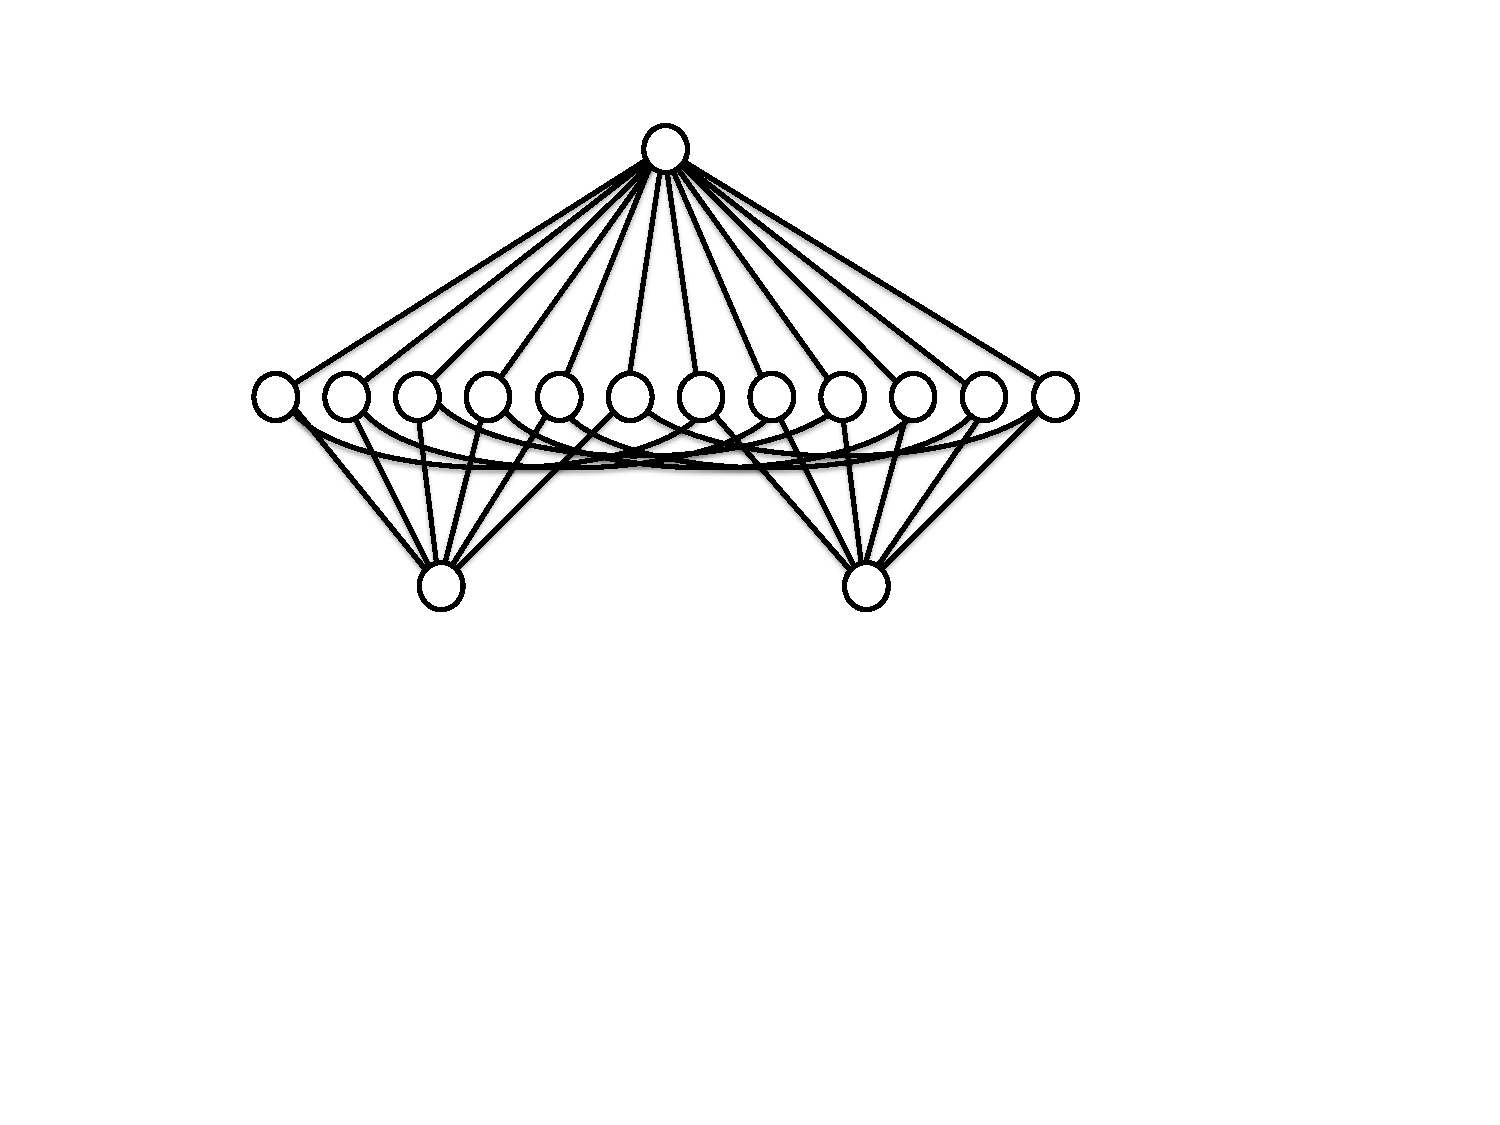
\includegraphics[height=8.0cm,width=9.0cm]{g15}
\vspace{-4cm}
\caption{Diamond-free $(12,6,6,3,3,3,3,3,3,3,3,3,3,3,3)$.}
\label{fig:g15}
\end{figure}
 
\begin{lemma} If $n=16$ and $\delta(1)=12$ then the degree sequence is either
\begin{enumerate}
\item $(12,12,9,3,3,3,3,3,3,3,3,3,3,3,3,3)$, or 
\vspace{-8pt}
\item $(12,12,6,6,3,3,3,3,3,3,3,3,3,3,3,3)$, or
\vspace{-8pt}
\item  $(12,9,9,6,3,3,3,3,3,3,3,3,3,3,3,3)$, or
\vspace{-8pt}
\item  $(12,6,3,3,3,3,3,3,3,3,3,3,3,3,3,3)$.
\end{enumerate}
\end{lemma}

\vspace{.25cm}
{\bf Proof} Let $u$ and $N(u)$ be defined as above, and let $v$, $w$ and $x$ be vertices that are not $u$
 and are not in $N(u)$, with corresponding degrees $\delta(v)\geq \delta(w)\geq \delta(x)$. By an argument similar to the above, $G$ has
 degree sequence $$(12,\delta(v),\delta(w),\delta(x),3,3,3,3,3,3,3,3,3,3,3,3)$$  where  $\delta(v)+\delta(w)+\delta(x)$ is divisible by $12$. 
Then we must have
 $(\delta(v),\delta(w),\delta(x))= (12,12,12)$, $(12,9,3)$, $(12,6,6)$ or $(9,9,6)$ or $(6,3,3)$. 
If $(\delta(v),\delta(w),\delta(x))=(12,12,12)$ then there are at least $3$
vertices in $N(u)$ that are adjacent to all of $u$, $v$, $w$ and $x$, which is impossible since, as before,
vertices in $N(u)$ must have degree $3$. In all other cases there are solutions (which we do not include here).

\chapter{Constraint Programming Models}
\label{sec:models}
\vspace{-3mm}
We present two constraint models for the diamond-free degree sequence problem. The first model we call
model A, the second model B. In many respects the two models are very similar but what is different
is how we solve them. In the subsequent descriptions we assume that we
have as input the integer $n$, where $|V| = n$ and vertex $i \in V$. All the constraint models were
implemented using the choco toolkit \cite{JChoco}. Further we assume that a variable $x$ has a domain of values
$dom(x)$.

\section{Model A}
\vspace{-3mm}
Model A is based on the adjacency matrix model of a graph.
We have a 0/1 constrained integer variable $A_{ij}$ for each potential edge in the graph such that 
$A_{ij} = 1 \iff \{i,j\} \in E$.
In addition we have constrained integer variables $deg_1$ to $deg_n$ corresponding to the
degrees of each vertex, such that
\begin{eqnarray}
\forall_{i \in [1..n]} ~ dom(deg_{i}) = [3~..~n-1]
\end{eqnarray}
We then have constraints to ensure that the graph is simple:
\begin{eqnarray}
\forall_{i \in [1..n]} \forall_{j \in [i .. n]} ~ A_{i,j} = A_{j,i} \\
\forall_{i \in [1..n]} ~ A_{i,i} = 0
\end{eqnarray}
Constraints are then required to ensure that the graph is diamond-free:
\begin{eqnarray}
\forall_{\{i,j,k,l\} \in V}~[A_{i,j} + A_{i,k} + A_{i,l} + A_{j,k} + A_{j,l} + A_{k,l} \leq 4]
\end{eqnarray}
Finally we have constraints on the degree sequence:
\begin{eqnarray}
\forall_{i \in [1~..~n]}~~deg_i = \sum_{j=1}^{j=n}A_{i,j}\\
\forall_{i \in [1~..~n-1]}~~deg_i \geq deg_{i+1} \\
\forall_{i \in [1~..~n]} ~~ deg_{i}~{\bf mod}~3 = 0 \\
\left({\sum_{i=1}^{i=n} deg_{i}}\right) ~{\bf mod}~12 = 0
\end{eqnarray}
The vertex degree variables $deg_1$ to $deg_n$ are the decision variables. The constraint model uses 
$O(n^{2})$ constrained integer variables and $O(n^{4})$ constraints.

\section{Model B}
\vspace{-3mm}
Model B is essentially model A broken into three parts, each part solved separately. The first part
is to produce a degree sequence that meets the arithmetic constraints. The second
part tests if that degree sequence is graphical and if it is the third part
determines if there exists a diamond-free graph with that degree sequence. Therefore solving proceeds
as follows.

\begin{enumerate}
\item Generate the next degree sequence $\pi = d_{1},d_{2},...,d_{n}$ that meets the arithmetical constraints.
If no more degree sequences exist then terminate the process.
\vspace{-8pt}
\item If the degree sequence $\pi$ is not graphical return to step 1.
\vspace{-8pt}
\item Determine if there is a diamond-free graph with the degree sequence $\pi$.
\vspace{-8pt} 
\item Return to step 1.
\end{enumerate}

The first part of model B is then as follows. Integer variables $deg_1$ to $deg_n$ correspond to the
degrees of each vertex and we satisfy constraints (1), (6), (7) and (8) to generate a degree sequence.

Each valid degree sequence produced is then tested to determine if it is graphical (step 2 above) using the 
Havel-Hakimi algorithm. We have used the $O(n^{2})$ algorithm \cite{hh} although the linear algorithm of \cite{hh2} 
could equally well be used and would have been more efficient. 

If the degree sequence is graphical (step 3) we create an adjacency matrix with properties
(2) and (3) and post the constraints (4) and (5) (diamond free with given degree sequence) where the variables $deg_{1}$ to $deg_{n}$ 
have already been instantiated (in step 1).
Finally we are in a position to post static symmetry breaking constraints. If we are producing a graph
and $deg_{i} = deg_{j}$ then these two vertices are interchangeable. Consequently we can insist that row $i$ in
the adjacency matrix is lexicographically less than or equal to row $j$. Therefore we post the symmetry breaking constraints:
\begin{eqnarray}
\forall_{i \in [1~..~n-1]}[deg_{i} = deg_{i+1} \Rightarrow A_{i} \preceq A_{i+1}]
\end{eqnarray}
where $\preceq$ means lexicographically less than or equal. In this second stage of solving the variables 
$A_{1,1}$ to $A_{n,n}$ are the decision variables.

\chapter{Solutions}
\label{sec:solutions}
\vspace{-3mm}
Our results are tabulated in Table \ref{tab1} for $8 \leq n \leq 16$. 
All our results are produced using model B run on a machine with 8 Intel Zeon E5420 processors 
running at 2.50 GHz, 32Gb of RAM, with version 5.2 of linux. The longest run time was for $n = 16$ taking about 5
minutes cpu time. Included in Table \ref{tab1} is the cpu time in seconds to generate all degree sequences for a given value of $n$.

\begin{table}
\begin{center}
\begin{tiny}
\begin{tabular}{|cc|l|} \hline 
  $n$  & time & degree sequence \\ \hline 
 8 & 0.1 & 3 3 3 3 3 3 3 3 \\ \hline
 9 & 0.1 & 6 6 6 3 3 3 3 3 3 \\ \hline
10 & 0.5 & 6 6 3 3 3 3 3 3 3 3 \\ \hline
11 & 0.8 & 6 3 3 3 3 3 3 3 3 3 3 \\ \hline
12 & 1.4 & 3 3 3 3 3 3 3 3 3 3 3 3 \\
   & & 6 6 6 6 3 3 3 3 3 3 3 3 \\
   & & 6 6 6 6 6 6 6 6 6 6 6 6  \\
   & & 9 6 6 3 3 3 3 3 3 3 3 3  \\ \hline
13 & 3.7 & 6 6 6 3 3 3 3 3 3 3 3 3 3  \\
   & & 6 6 6 6 6 6 6 3 3 3 3 3 3  \\
   & & 6 6 6 6 6 6 6 6 6 6 6 3 3  \\
   & & 9 6 3 3 3 3 3 3 3 3 3 3 3  \\ \hline
14 & 14.0 & 6 6 3 3 3 3 3 3 3 3 3 3 3 3 \\ 
   & & 6 6 6 6 6 6 3 3 3 3 3 3 3 3 \\
   & & 6 6 6 6 6 6 6 6 6 6 3 3 3 3 \\
   & & 6 6 6 6 6 6 6 6 6 6 6 6 6 6 \\
   & & 9 3 3 3 3 3 3 3 3 3 3 3 3 3 \\
   & & 9 6 6 6 6 3 3 3 3 3 3 3 3 3 \\
   & & 9 9 6 6 3 3 3 3 3 3 3 3 3 3 \\
   & & 9 9 9 3 3 3 3 3 3 3 3 3 3 3 \\ \hline
15 & 107.7 & 6 3 3 3 3 3 3 3 3 3 3 3 3 3 3 \\
   & & 6 6 6 6 6 3 3 3 3 3 3 3 3 3 3 \\
   & & 6 6 6 6 6 6 6 6 6 3 3 3 3 3 3 \\
   & & 6 6 6 6 6 6 6 6 6 6 6 6 6 3 3 \\
   & & 9 6 6 6 3 3 3 3 3 3 3 3 3 3 3 \\
   & & 9 6 6 6 6 6 6 6 3 3 3 3 3 3 3 \\
   & & 9 6 6 6 6 6 6 6 6 6 6 6 3 3 3 \\
   & & 9 9 6 3 3 3 3 3 3 3 3 3 3 3 3 \\
   & & 9 9 6 6 6 6 6 3 3 3 3 3 3 3 3 \\
   & & 9 9 6 6 6 6 6 6 6 6 6 3 3 3 3 \\
   & & 9 9 9 6 6 6 3 3 3 3 3 3 3 3 3 \\
   & & 9 9 9 9 9 9 6 6 6 6 6 6 6 6 6 \\
   & & 12 6 6 3 3 3 3 3 3 3 3 3 3 3 3 \\
   & & 12 12 12 3 3 3 3 3 3 3 3 3 3 3 3 \\ \hline
16 & 339.8 & 3 3 3 3 3 3 3 3 3 3 3 3 3 3 3 3 \\
   & & 6 6 6 6 3 3 3 3 3 3 3 3 3 3 3 3 \\
   & & 6 6 6 6 6 6 6 6 3 3 3 3 3 3 3 3 \\
   & & 6 6 6 6 6 6 6 6 6 6 6 6 3 3 3 3 \\
   & & 6 6 6 6 6 6 6 6 6 6 6 6 6 6 6 6 \\
   & & 9 6 6 3 3 3 3 3 3 3 3 3 3 3 3 3 \\
   & & 9 6 6 6 6 6 6 3 3 3 3 3 3 3 3 3 \\
   & & 9 6 6 6 6 6 6 6 6 6 6 3 3 3 3 3 \\
   & & 9 9 3 3 3 3 3 3 3 3 3 3 3 3 3 3 \\
   & & 9 9 6 6 6 6 3 3 3 3 3 3 3 3 3 3 \\
   & & 9 9 6 6 6 6 6 6 6 6 3 3 3 3 3 3 \\
   & & 9 9 6 6 6 6 6 6 6 6 6 6 6 6 3 3 \\
   & & 9 9 9 6 6 3 3 3 3 3 3 3 3 3 3 3 \\
   & & 9 9 9 6 6 6 6 6 6 6 6 6 6 3 3 3 \\
   & & 9 9 9 9 3 3 3 3 3 3 3 3 3 3 3 3 \\
   & & 9 9 9 9 6 6 6 6 6 6 6 6 3 3 3 3 \\
   & & 9 9 9 9 6 6 6 6 6 6 6 6 6 6 6 6 \\
   & & 9 9 9 9 9 6 6 6 6 6 6 6 6 6 6 3 \\
   & & 9 9 9 9 9 9 6 6 6 6 6 6 6 6 3 3 \\
   & & 12 6 3 3 3 3 3 3 3 3 3 3 3 3 3 3 \\
   & & 12 9 9 6 3 3 3 3 3 3 3 3 3 3 3 3 \\
   & & 12 12 6 6 3 3 3 3 3 3 3 3 3 3 3 3 \\
   & & 12 12 9 3 3 3 3 3 3 3 3 3 3 3 3 3 \\ \hline
\end{tabular}
\end{tiny}
\end{center}
\caption{Degree sequences, of length $n$, that meet the arithmetic constraints and have a simple diamond-free graph. Tabulated
is $n$, cpu time in seconds to generate all sequences of length $n$ and those sequences.}
\label{tab1}
\end{table}

All our results were verified. For each degree sequence the corresponding adjacency matrix 
was saved to file and verified to correspond to a simple diamond-free graph that matched the degree sequence and 
satisfied the arithmetic constraints and this is an $O(n^{4})$ process. The verification software did not use 
any of the constraint programming code.

\chapter{Conclusion}
\label{sec:conc}
\vspace{-3mm}
We have presented a new problem, the generation of all degree sequences for diamond free
graphs subject to arithmetic constraints. Two models have been presented, A and B. Model A is
impractical whereas model B is two stage and allows static symmetry breaking.

There are two possible improvements. The first is to model A. We might add the lexicographical
constraints, as used in model B, conditionally during search. The second improvement worthy
of investigation is to employ a mixed integer programming solver for the second stage 
of model B.

We are currently using the lists of feasible degree sequences for
diamond-free graphs with $15$ or $16$ vertices to simplify our proofs
for the classification of $4^{s_{4}}$ structures with diamond-free
complements, when the number of points in the maximum number of blocks
is $1$ or $0$ respectively. The degree sequence results for a smaller
number of points will also help to simplify our existing proofs for
cases where more points are in the maximum number of
blocks. Ultimately we would like to use our classification to modify
the extension of Stinson's algorithm for block size $4$ to ensure that
a block design is always produced. 

In the more distant future, we would like to analyse the structures
produced using our algorithm when $n>16$. The next case is $n=25$ and
the corresponding diamond-free graphs would have up to $25$
vertices.

\section*{Acknowledgments}
\label{sec:ack}
\vspace{-3mm}
We would like to thank Ian Miguel for his help in setting up the original CSPLib problem \cite{CSPLib},  and Mike Codish and Brendan McKay for pointing out errors in an earlier draft of this paper.


\bibliographystyle{plain}
\bibliography{bib}

\end{document}




